% ════════════════════════════════════════════
% 5. 数据分析
% ════════════════════════════════════════════
\section{数据分析}

\subsection{样本结构与分组对比}

图\ref{fig:structure}从三个角度补充样本结构。左上背靠背条形把类型与付费拆开：Photo 在两组中都占 85\% 以上（自然 307 条、付费 119 条），Status 与 Link 合计不足 15\%，Video 只有 7 条且其中 4 条付费，说明类型效应主要由 Photo 与 Status 支撑，Video 的估计必然带有较大不确定性。右上半小提琴图给出三类主题的曝光分布，中位数分别为 9.25、9.09、9.02（对数尺度），三组重叠很大，单看主题不足以区分帖子表现。下方联合密度图的散点呈近竖直云团，粉丝规模对数与曝光对数的 Pearson 相关仅 $-0.082$（$p=0.066$），上缘与右缘的边缘直方图进一步显示两组在粉丝规模上几乎重合、在曝光轴上付费组整体右移。

\begin{figure}[htbp]
  \centering
  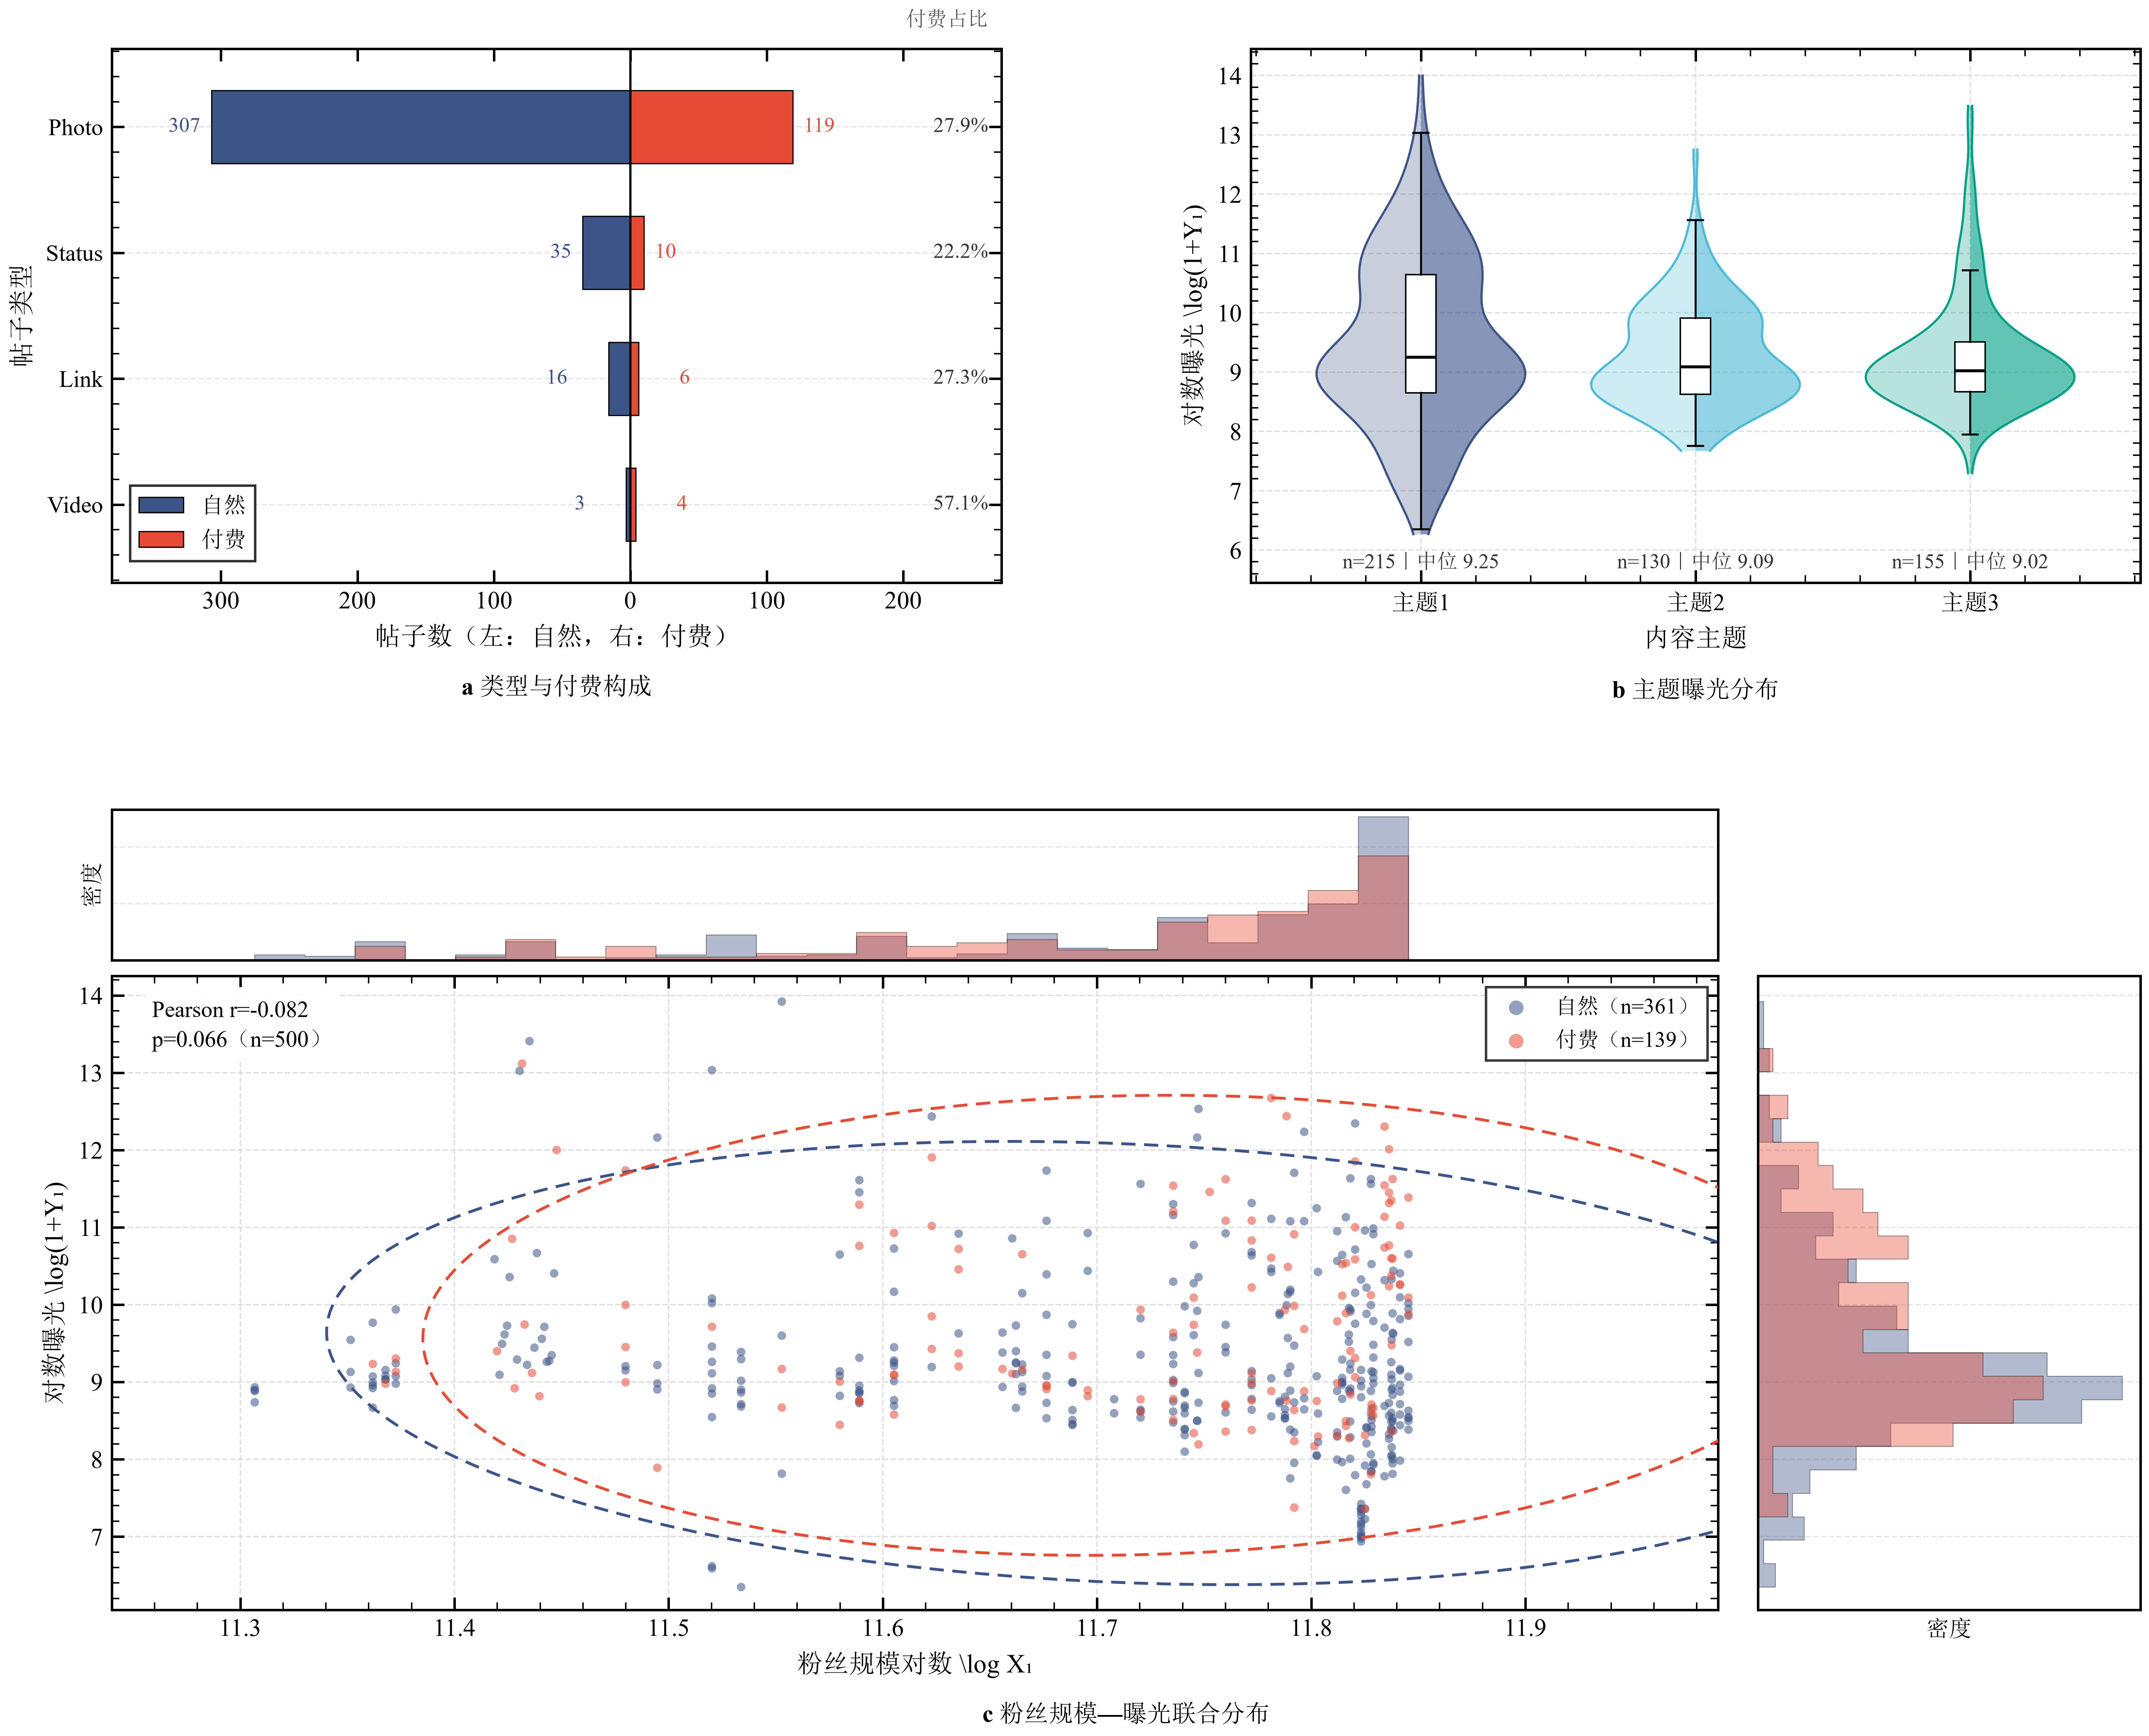
\includegraphics[width=0.63\textwidth]{../求解/临时产物/补充图1_样本结构.png}
  \caption{样本构成、主题分布与粉丝—曝光联合分布}
  \label{fig:structure}
\end{figure}

\subsection{变量与曝光的关联强度}

图\ref{fig:corr}的下三角气泡矩阵给出七个变量的两两 Spearman 相关。与曝光关系最强的是付费（0.171），其余依次为内容主题（$-0.080$）、星期（$-0.071$）、月份与粉丝规模（均为 $-0.135$），方向虽为负但幅度都很小；矩阵中最突出的一格是粉丝规模与月份（0.996，黑圈标注），这正是第 4.3 节判定不可同时识别的依据。右侧条形把各变量与曝光的相关系数单独列出，全部落在 $\pm0.20$ 以内，说明没有单一变量能解释曝光差异，这也是必须使用多元回归而非单变量比较的原因。

\begin{figure}[htbp]
  \centering
  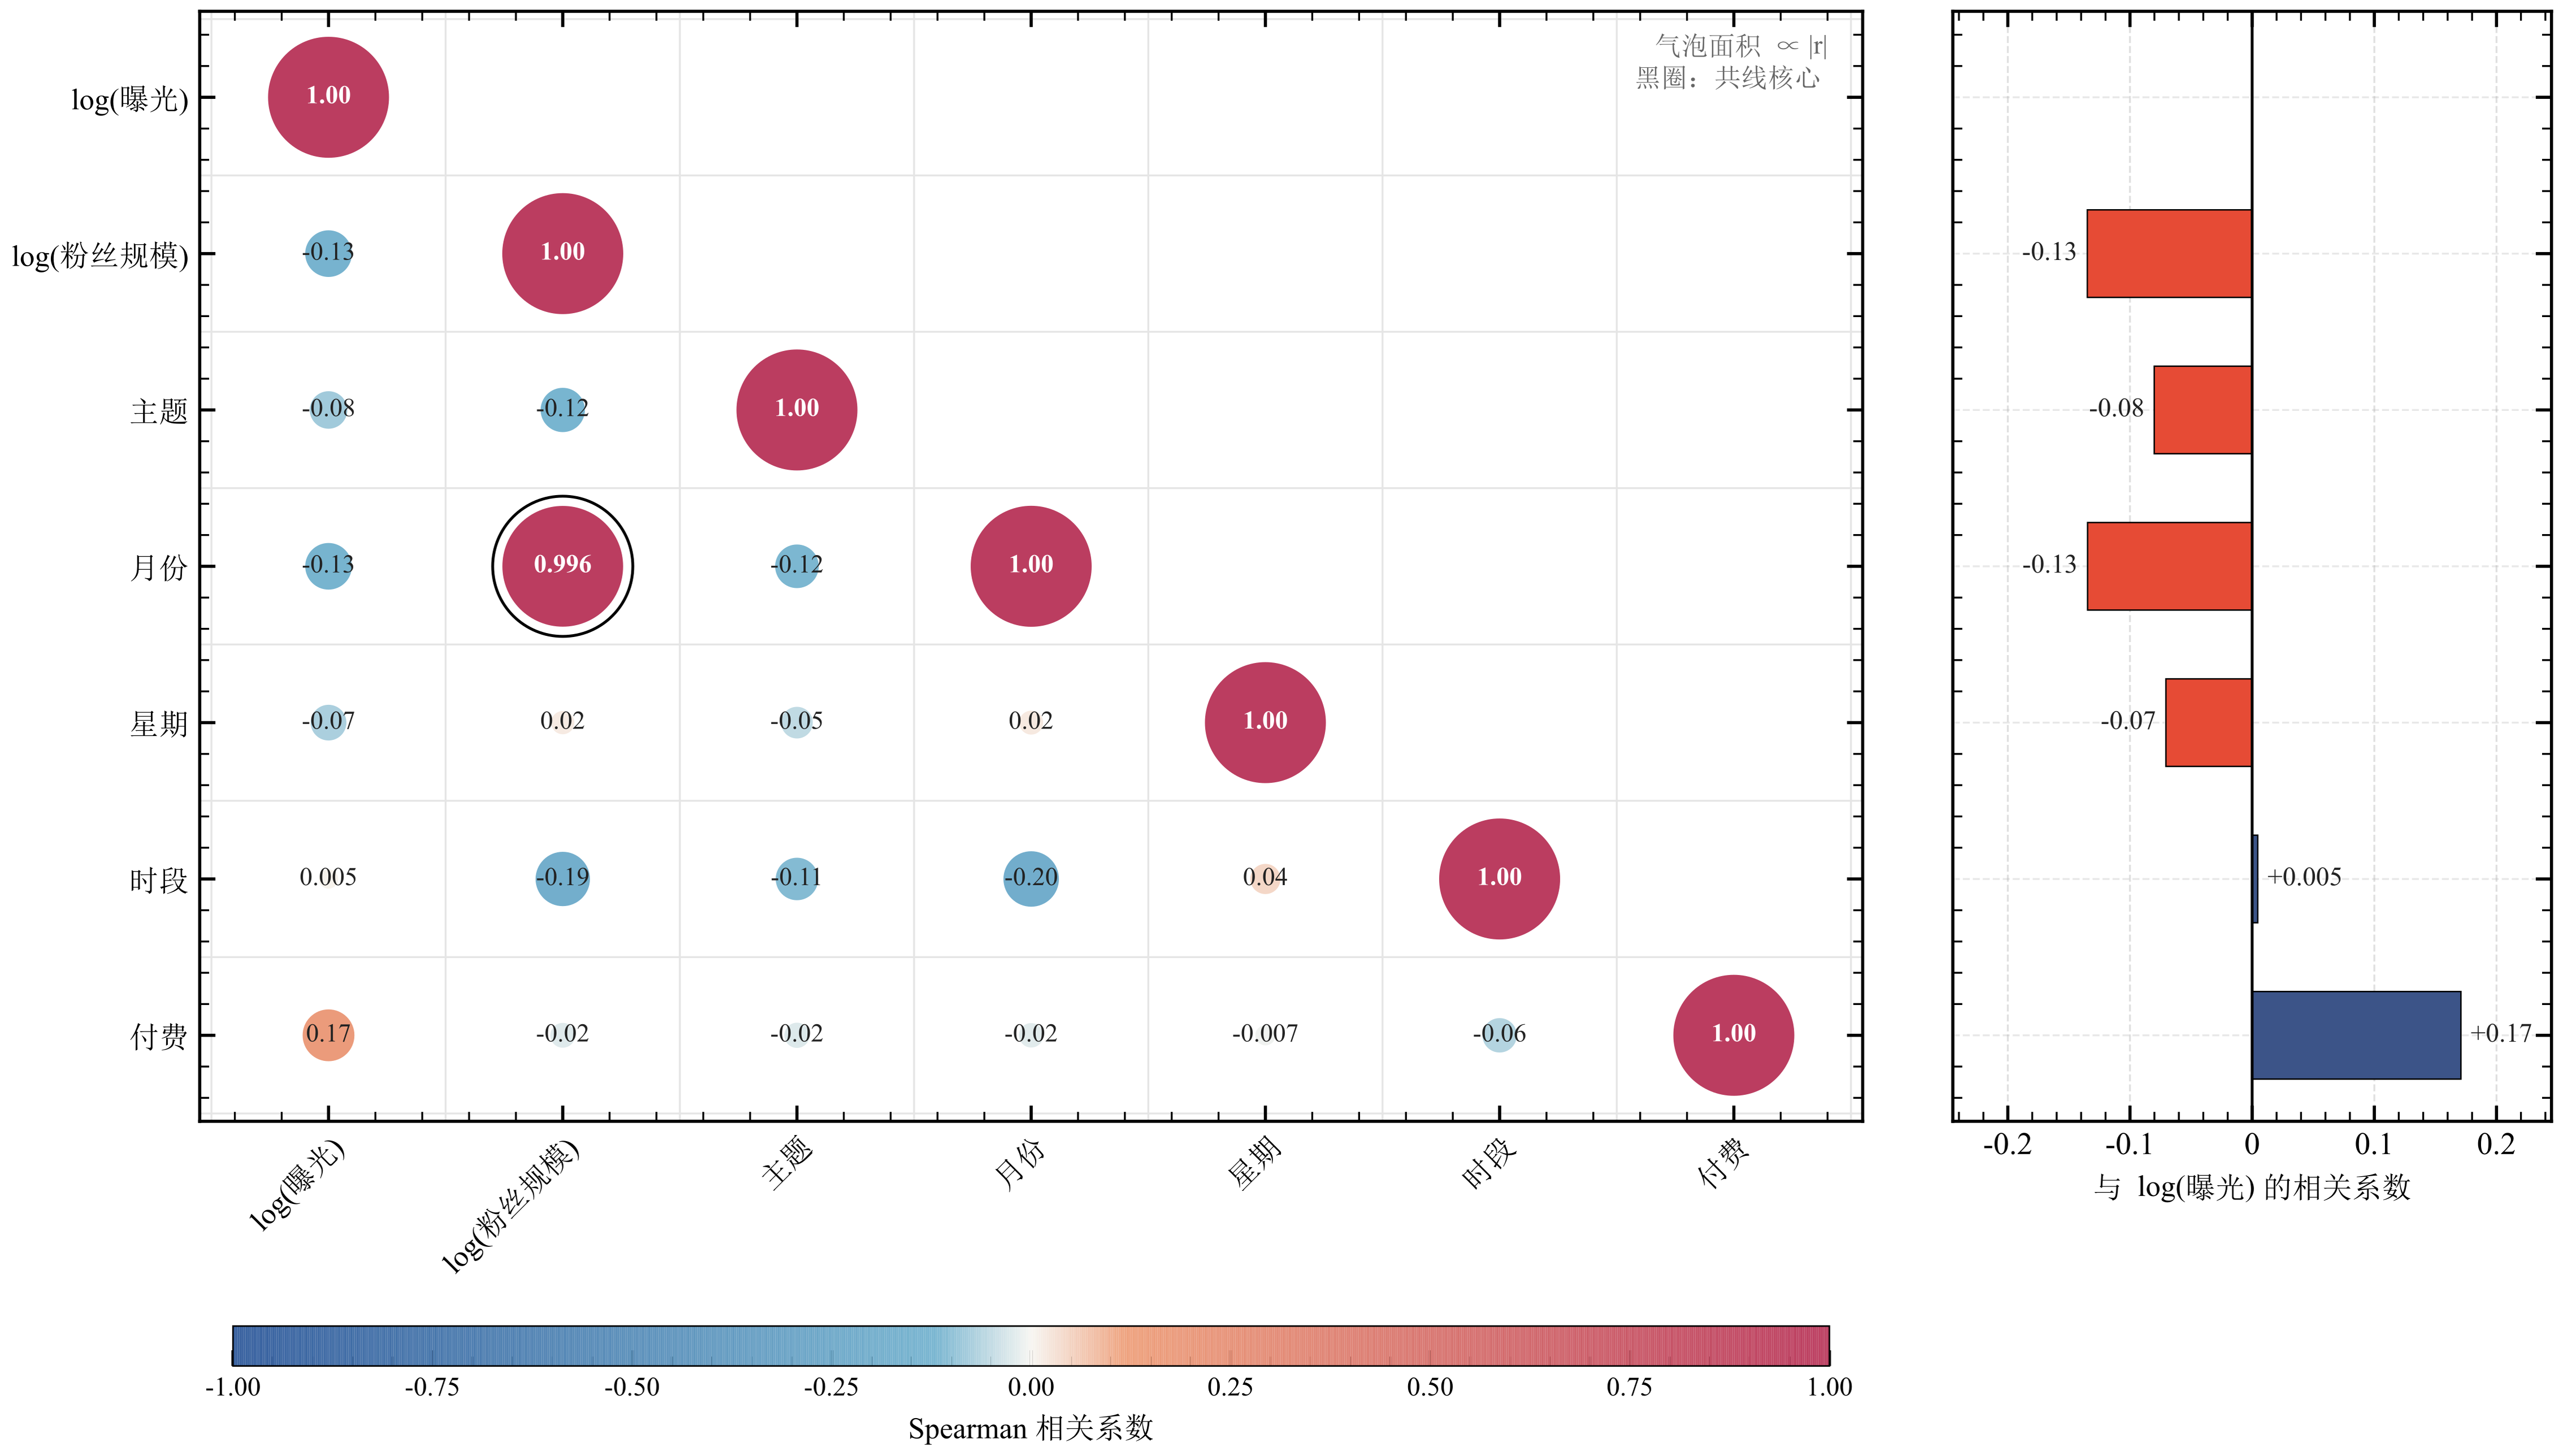
\includegraphics[width=0.70\textwidth]{../求解/问题一/结果/图3_相关系数热力图.png}
  \caption{变量间的 Spearman 相关矩阵与各变量对曝光的相关强度}
  \label{fig:corr}
\end{figure}

\subsection{时间维度的差异}

左上月度柱线图显示发帖量在 10 月最高（60 条）、1 月最低（25 条），付费占比在 4 月达到 40.0\%、1 月仅 16.0\%，整体为 27.8\%；右上月度均值曲线的最高点出现在 2 月（10.13）、最低点在 10 月（8.83），说明发帖量与平均曝光并不同步。下方两张误差棒图给出星期与时段差异：星期四的平均对数曝光最高（9.74）、星期日最低（9.06），下午晚间最高（9.50）、上午最低（9.25）。这些差异幅度有限，且与月份的分布纠缠，因此不单独解读，交由回归在控制其他变量后估计。


